\let\negmedspace\undefined
\let\negthickspace\undefined
\documentclass[journal,12pt,twocolumn]{IEEEtran}
\usepackage{cite}
\usepackage{amsmath,amssymb,amsfonts,amsthm}
\usepackage{algorithmic}
\usepackage{graphicx}

\usepackage{textcomp}
\usepackage{xcolor}
\usepackage{txfonts}
\usepackage{listings}
\usepackage{enumitem}
\usepackage{mathtools}
\usepackage{gensymb}
\usepackage{comment}
\usepackage[breaklinks=true]{hyperref}
\usepackage{tkz-euclide} 
\usepackage{listings}
\usepackage{gvv}                                                                      
\usepackage[latin1]{inputenc}                                
\usepackage{color}                                            
\usepackage{array}                                            
\usepackage{longtable}                                       
\usepackage{calc}                                             
\usepackage{multirow}                                         
\usepackage{hhline}                                           
\usepackage{ifthen}                                           
\usepackage{lscape}
\setlength{\arrayrulewidth}{0.5mm}
\setlength{\tabcolsep}{18pt}
\renewcommand{\arraystretch}{1.5}
\newtheorem{theorem}{Theorem}[section]
\newtheorem{problem}{Problem}
\newtheorem{proposition}{Proposition}[section]
\newtheorem{lemma}{Lemma}[section]
\newtheorem{corollary}[theorem]{Corollary}
\newtheorem{example}{Example}[section]
\newtheorem{definition}[problem]{Definition}
\newcommand{\BEQA}{\begin{eqnarray}}
\newcommand{\EEQA}{\end{eqnarray}}
\newcommand{\define}{\stackrel{\triangle}{=}}
\theoremstyle{remark}
\newtheorem{rem}{Remark}
\begin{document}

\bibliographystyle{IEEEtran}
\vspace{3cm}

\title{ANALOG 12.8 8}
\author{EE23BTECH11054 - Sai Krishna Shanigarapu$^{*}$% <-this % stops a space
}
\maketitle
\newpage
\bigskip

\begin{flushleft}
\textbf{Question 8:}\\
Suppose that the electric field amplitude of an electromagnetic wave is $E_0$ = 120N/C and that its frequency is $f$ = 50.0 MHz.\\
(a) Determine, $B_0, \omega, k$ and $\lambda$\\
(b) Find expressions for \textbf{E} and \textbf{B}\\
\end{flushleft}

\bigskip

\begin{flushleft}
\textbf{Solution (a):}\\
\end{flushleft}

\begin{center}
    \begin{table}[h]
        \caption{Input Parameters}
        \setlength{\arrayrulewidth}{0.3mm}
\setlength{\tabcolsep}{18pt}
\renewcommand{\arraystretch}{1.5}

\textbf{Table 1 - Input parameters}\\

\begin{tabular}{ |p{1cm}|p{1cm}|p{1.7cm}|  }
\hline
\multicolumn{3}{|c|}{Input Parameters} \\
\hline
Symbol& Description&value\\
\hline
$f$ & frequency of source & 50.0 MHz\\
\hline
$E_0$ & Electric field amplitude  & 120 N/C\\
\hline
$c$ &speed of light & 3 x 10$^8$ m/s \\
\hline
\end{tabular}
    
        \label{tab:table1.12.8.8}
    \end{table}
\end{center}

\begin{flushleft}
   General representation of electric and magnetic field is:\\
   \begin{align}
   \vec{E} = E_0sin(kx - \omega t)\vec{e_2}\\
   \vec{B} = B_0sin(kx - \omega t)\vec{e_3}
   \end{align}

   \begin{align}
    B_0 = \frac{E_0}{c} = \frac{120}{3 x 10^8} = 400nT\\
    \omega = 2\pi f = 3.14 x 10^8 rad/s\\
    k = \frac{\omega}{c} = 1.05 rad/m\\
    \lambda = \frac{c}{f} = \frac{3 x 10^8}{50 x 10^6} = 6.0m    
    \end{align}

\bigskip

    \textbf{Solution (b):}\\
    \bigskip
    from the above equations, \\
    \begin{align}
    \vec{E} &= 120 sin[1.05x - 3.1 x 10^8t]\vec{e_2}\\
    \vec{B} &= (4 x 10^{-7})sin[1.05x - 3.14 x 10^8t]\vec{e_3}
    \end{align} 
\end{flushleft}

\bigskip

\begin{center}
    \begin{table}[h]
        \caption{Output Parameters}
        \setlength{\arrayrulewidth}{0.3mm}
\setlength{\tabcolsep}{15pt}
\renewcommand{\arraystretch}{1.5}

\begin{center}
\begin{tabular}{ |p{1cm}|p{1cm}|p{4.5cm}|  }
\hline
\multicolumn{3}{|c|}{Output parameters} \\
\hline
Symbol& Description&value\\
\hline
$B_0$ & Magnetic field strength & 400nT\\
\hline
$\omega$ & Angular frequency & 3.14 x 10$^8$m/s\\
\hline
$k$ &Propagation constant & 1.05rad/s\\
\hline
$\lambda$ & Wavelength & 6.0m\\
\hline
$\vec{E}$ & Electric field vector & 120 sin[1.05x - 3.1 x 10$^8$t]$\vec{e_2}$\\
\hline
$\vec{B}$ & Magnetic field vector & (4 x 10$^{-7}$)sin[1.05$x$ - 3.14 x 10$^8$t]$\vec{e_3}$\\
\hline
\end{tabular}
\end{center}
        \label{tab:table2.12.8.8}
    \end{table}
\end{center}

\renewcommand{\thefigure}{\theenumi}
\renewcommand{\thetable}{\theenumi}

\newpage

\begin{center}
\begin{figure}[h]
\renewcommand\thefigure{1}
  \caption{Graphs of $\vec{E}$ and $\vec{B}$}
  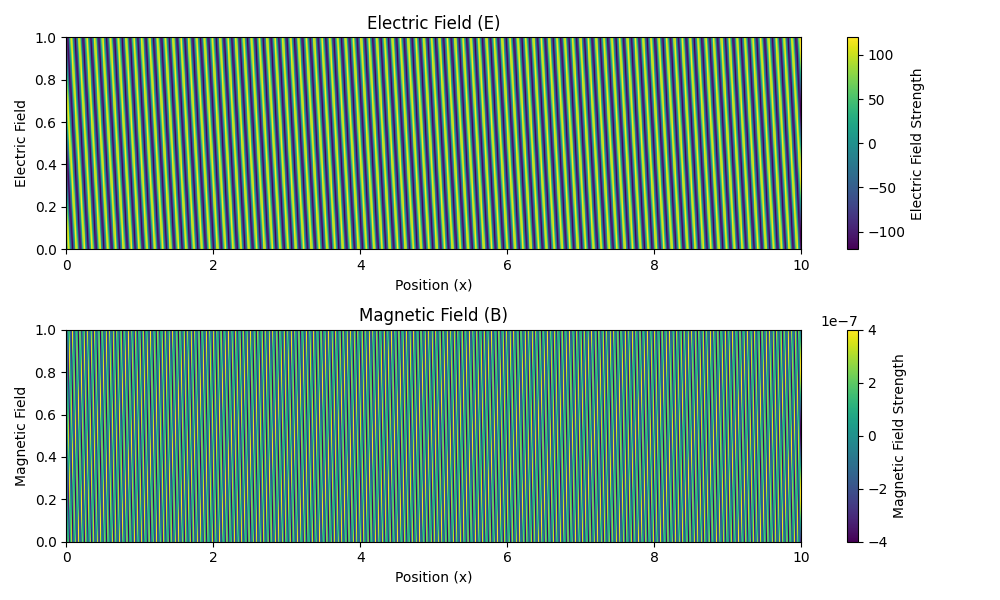
\includegraphics[width=1\textwidth]{figs/Figure1_12.8_8.png}
  \label{fig:graphs}
\end{figure}
\end{center}

\end{document}
